\documentclass{article}
\usepackage{tikz}
\usepackage{amsmath}

\begin{document}
\pagenumbering{gobble}

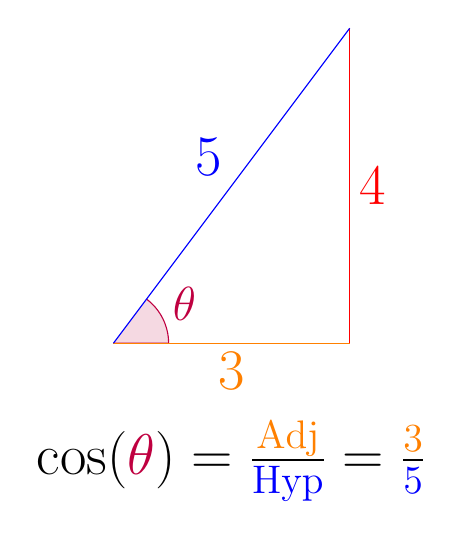
\begin{tikzpicture}

\filldraw[color=purple!100, fill=purple!15] (0,0) -- (.7,0) arc(0:53.13:.7);
\draw (.9, .5) node {\LARGE \textcolor{purple}{$\theta$}};

\draw [orange] (0,0) -- node[below] {\huge \textcolor{orange}{3}} (3,0);
\draw [red] (3,0) -- node[right] {\huge \textcolor{red}{4}} (3,4);
\draw [blue] (3,4) -- node[above left] {\huge \textcolor{blue}{5}} (0,0);


\draw (1.5, -1.5) node {\huge $\cos(\textcolor{purple}{\theta}) = \frac{\textrm{\textcolor{orange}{Adj}}}{\textrm{\textcolor{blue}{{Hyp}}}} = \frac{\textcolor{orange}{\textrm{3}}}{\textcolor{blue}{\textrm{5}}}$};

\end{tikzpicture}
\end{document}